\section{The interaction is regime-scoped}
\label{sec:regime}

A reader could take \S\ref{sec:interaction} as ``look-ahead does not work with preference
trees.'' That reading is testable, because the lever has a history: \citet{baruch2025pto}
reported it \emph{helping} a preference-tree therapist in an earlier regime of the same task ---
a 7B therapist, a more cooperative patient population, a weaker grader, and non-iterative
training. Rather than trust the two papers' incomparable score axes, we re-scored the earlier
regime's conversations directly.

\textbf{Re-scored under the modern grading stack, the earlier regime still shows a
preference-tree look-ahead gain.} Across the seven training iterations of the earlier
experiment, the $\Kf$ models outscore the $\Kz$ models on the same conversations by $+0.132$ on
average (\dz\,$0.543$, $p < .001$, persona-paired) under the modern oracle, and by $+0.206$
(\dz\,$0.612$) under a grader matched to the original paper's; best-vs-best, the $\Kf$ arm's
peak beats the $\Kz$ arm's peak under the modern oracle ($+0.129$, \dz\,$0.250$, $p = .006$)
(Figure~\ref{fig:crossgen}). The original result was real, and it was not an artifact of the
original judge.

\begin{figure}[t]
\centering
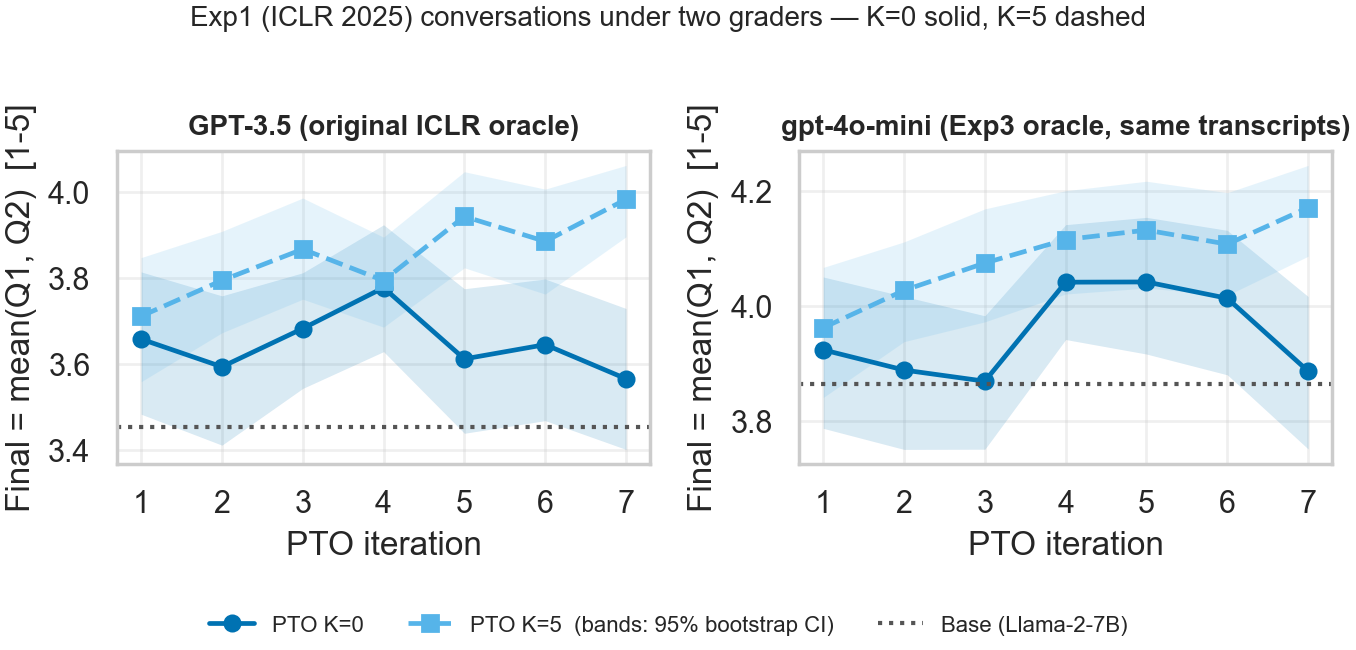
\includegraphics[width=0.98\linewidth]{figures/crossgen.png}
\caption{The earlier regime's conversations re-scored: \QQ-style score by iteration for its
$\Kz$ and $\Kf$ preference-tree arms, under the modern oracle and under a grader matched to the
original study. Look-ahead wins in that regime under both --- the same lever whose outcome
effect is null for \PTO\ in the present regime.}
\label{fig:crossgen}
\end{figure}

\textbf{So the null is a property of the regime, not the lever--optimizer pairing as such.} The
same lever, same optimizer family, same task: positive in the easy regime, null on outcomes in
the hard one --- while in the hard regime the same lever transforms a different optimizer. At
least three regime ingredients plausibly matter and are confounded with each other here: the
policy scale (7B vs.\ 1B), the patient difficulty (cooperative vs.\ resistant personas), and the
training loop (static vs.\ iterative self-generated data). This experiment cannot separate them;
what it can establish is the methodological point, which survives any of those attributions:
\textbf{a reward-design lever's sign is not portable across optimizers or regimes, and papers
reporting such levers on one optimizer in one regime are reporting an interaction cell, not a
main effect.}
